\chapter{METODOLOGÍA DE LA INVESTIGACIÓN}
\section{Diseño de la investigación}
En esta sección del documento se explica cuál fue el diseño, el tipo y el enfoque del trabajo de investigación, así como también la población y la muestra. 

\subsection{Tipo de la investigación}
Para determinar el tipo de la investigación, primero fue necesario definir el actual trabajo como Diseño Experimental ya que, según \cite{bk_hernandez2014metodologia} en su libro \citetitle{bk_hernandez2014metodologia}, se pretende establecer el posible efecto de una causa que se manipula. Dentro de esta categoría se clasifica como Diseño Experimental Puro, ya que se manipuló intencionalmente más de una variable independiente (fueron agregadas y/o removidas) con la finalidad de medir el efecto que estas generan en la variable dependiente, el estado final de financiamiento de un proyecto de tecnología en Kickstarter.

\subsection{Enfoque de la investigación}
El presente trabajo tuvo un enfoque cuantitativo ya que, según \cite{bk_hernandez2014metodologia} en su libro \citetitle{bk_hernandez2014metodologia}, este enfoque utiliza la recolección de datos para probar hipótesis con base en la medición numérica y el análisis estadístico, con el fin de establecer pautas de comportamiento y probar teorías. Esto se refleja en los 10 pasos del proceso cuantitativo descritos por el anterior autor y que fueron aplicados en la investigación, desde la concepción de la idea hasta la elaboración del reporte de resultados.

\subsection{Población}
La población fueron todos los proyectos de la web de crowdfunding Kickstarter.

\subsection{Muestra}
La muestra fueron 27,251 proyectos, incluyendo exitosos y fracasados, de la categoría Tecnología, de la web de crowdfunding Kickstarter, entre los periodos 2009 y 2019. Como se mencionó en el Capítulo I, el criterio de la elección de esta categoría se debe a su bajo ratio de éxito de financiamiento en promedio durante los periodos mencionados, los cuales se consideraron hasta el 2019 dado que tomar el año 2020 incurriría en la distorsión del ratio por la coyuntura de la pandemia del Covid-19.

\subsection{Operacionalización de Variables}
En la Tabla \ref{3:table1} se presenta la operacionalización de variables para la investigación.

%\begin{table}[h!]

\begin{longtable}{|M{5cm}|M{4.5cm}|M{5.5cm}|}
	\caption[Matriz de operacionalización de variables]{Matriz de operacionalización de variables.}
	\label{3:table1}
	\newcommand{\multirot}[1]{\multirow{2}{*}[-8ex]{\rotcell{\rlap{#1}}}}
	\centering
	\small
	\tabularnewline\hline
	\textbf {VARIABLE} & \textbf {INDICADOR} & \textbf {CÁLCULO}
	\\%%[5pt]
	\hline
	\multirow{2}{5cm}[-2ex]{\centering Estado de financiamiento de un proyecto} & Proyecto exitoso & Monto meta $\leq$ monto contribuido                                                   \\%%[10pt]
	\cline{2-3} & Proyecto fracasado & Monto meta $>$ monto contribuido \\%%[10pt]
	\hline
	\multirow{2}{5cm}[-6ex]{\centering Aprendizaje Profundo Multimodal} & Modelo de Aprendizaje Profundo & \setlist{nolistsep}
	\begin{itemize}[noitemsep,leftmargin=*]
		\item Perceptrón Multicapa
		\item Red Neuronal Convolucional
		\item LSTM Bidireccional
	\end{itemize} \\
	\cline{2-3} 
	& Procesamiento de Lenguaje Natural &
	\setlist{nolistsep}
	\begin{itemize}[noitemsep,leftmargin=*]
		\item Pre-procesamiento de textos
		\item Representación de textos en vectores
	\end{itemize} \\
	\hline
	\multirow{5}{5cm}{\centering Efectividad del modelo} & Exactitud & $\frac{V.P.+V.N.}{V.P.+V.N.+F.P.+F.N.}$ \\%%[10pt]
	\cline{2-3} 
	& Precisión & $\frac{V.P.}{V.P.+F.P.}$ \\%%[10pt]
	\cline{2-3} 
	& Área bajo la curva ROC & $P( score(x^{+}) > score(x^{-}) )$ \\%%[10pt]
	\cline{2-3} 
	& Sensibilidad & $\frac{V.P.}{V.P.+F.N.}$ \\%%[10pt]
	\cline{2-3} 
	& Puntaje F1 & $\frac{2*Precisi\acute{o}n*Sensibilidad}{Precisi\acute{o}n+Sensibilidad}$ \\%%[10pt]
	\hline
\end{longtable}
%\par	%%Salto de linea
%\bigskip
\begin{flushleft}	%%Alinear a la izquierda sin justificar
	\small Fuente: Elaboración propia.
\end{flushleft}
%\end{table}

El trabajo busca resolver el problema de clasificación del estado final de financiamiento de un proyecto a través de la implementación de un modelo de Aprendizaje Profundo Multimodal.

Como se explica en la subsección 2.3.3, un proyecto de Kickstarter presenta 5 categorías de acuerdo al logro del objetivo de su meta: exitoso, fracasado, vigente, suspendido y cancelado. Dado que se busca predecir si, a partir de una serie de variables, el proyecto llegará a ser financiado o no, el estudio se delimita a estas 2 clases. Para determinar este valor, y según la política “Todo o Nada” de la plataforma explicado en la subsección 2.3.2, un proyecto es determinado como exitoso cuando el monto contribuido al culminar el tiempo de vida de su campaña logra ser mayor o igual a su meta estimada. De lo contrario, se dice que es un proyecto fracasado.

Con el fin de alcanzar el objetivo, se utilizó como principal vehículo un modelo de Aprendizaje Profundo Multimodal, cuyo concepto teórico se explica en la Sección 2.2.4. Este modelo, alimentado de 3 modalidades independientes presentes en cada campaña de Kickstarter, comprende el ensamblaje de 3 modelos de Aprendizaje Profundo: un modelo Perceptrón Multicapa (MLP), una Red Neuronal Convolucional (CNN) y un modelo LSTM Bidireccional. Al mismo tiempo, para los 2 últimos que corresponden a las modalidades de descripción y comentarios respectivamente, se trabajaron sus datos de entrada con técnicas de Procesamiento de Lenguaje Natural que incluye desde el pre-procesamiento de los textos hasta su conversión en vectores que finalmente serán entrenados.

Por último, para poder evaluar la efectividad que este registrará al ser entrenado, su desempeño será evaluado a través de métricas de clasificación de Minería de Datos. Para la investigación, las 5 métricas utilizadas fueron la exactitud, la precisión, el área bajo la curva ROC, la sensibilidad y el puntaje F1, las cuales se describen en la Sección 2.2.9.
%\clearpage

\section{Técnicas de recolección de datos}
Los conjuntos de datos recolectados para la investigación se componen de mezcla de observaciones cuantitativas (variables numéricas basadas en características del proyecto como la meta de financiamiento, montos prometidos, duración de la campaña y otros indicadores financieros) y cualitativas (descripción y comentarios del proyecto). Para obtener los 3 principales datasets, se siguió el flujo de la Figura \ref{3:fig1}. La base de datos de la metainformación, que comprende las variables cuantitativas y propaganda del proyecto, fue consolidada luego de descargar un histórico público de 10 años de la página web “Web Robots”, fundada por los ex corporativos de TI Tomás Vitulskis y Paulius Jonaitis, y posteriormente pre-procesarla. Mientras que por el lado de la descripción y comentarios de cada proyecto, se usaron técnicas y herramientas de \textit{web scraping} a partir de los URLs.

\begin{figure}[h]
	\begin{center}
		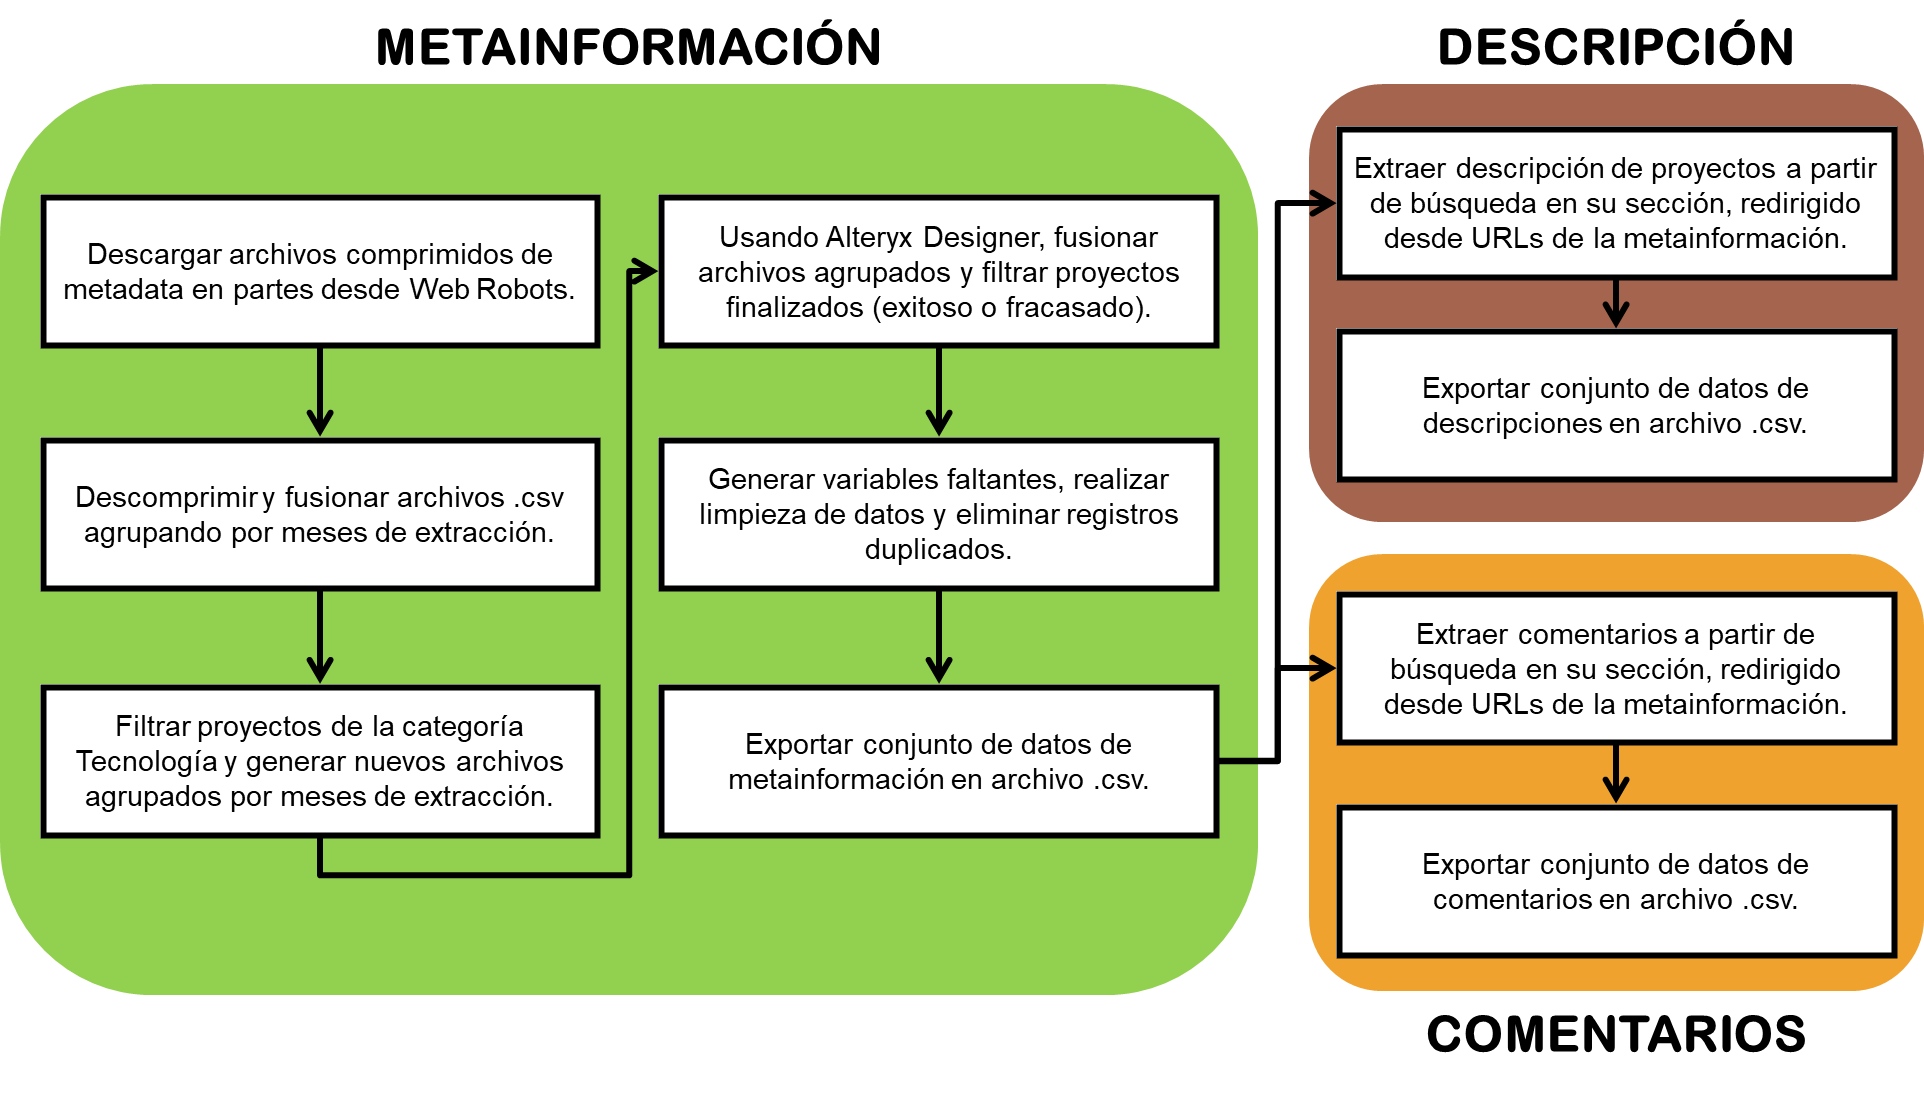
\includegraphics[width=1\textwidth]{3/figures/data_recolection_flux.png}
		\caption[Flujograma de la recolección de conjuntos finales de datos]{Flujograma de la recolección de conjuntos finales de datos.\\
			Fuente: Elaboración propia.}
		\label{3:fig1}
	\end{center}
\end{figure}

Asimismo, para encontrar algunos de los papers con la información requerida más cercana, se utilizaron keywords o palabras clave como \textit{crowdfunding}, \textit{Machine Learning}, \textit{Deep Learning}, \textit{prediction}, \textit{Kickstarter}, \textit{accuracy} y \textit{projects}.

\section{Técnicas para el procesamiento y análisis de la información}

\subsection{Metodología de implementación de la solución}
Como se explicó en el punto 2.2.6 del Marco Teórico del presente trabajo, según \cite{tec_braulio2015metodologiasdm}, dentro de los sistemas de analítica de negocio, Big Data y Minería de Datos, tres de las metodologías más usadas son CRISP-DM, SEMMA y KDD. Los mismos autores detallan en la Tabla \ref{2:table1} las características que cada una presenta al compararse.

Para escoger la metodología, se elaboró la Tabla \ref{3:table2} con el fin de comparar las utilizadas por los autores en los antecedentes. 17 de los 18 autores implementaron sus propias metodologías, las cuales de acuerdo a su similitud se agruparon en 8 grupos.

%\begin{table}[htbp]
\begingroup
	\renewcommand\arraystretch{0.3}
	\begin{longtable}{|M{3cm}|M{2.5cm}|M{2.5cm}|M{6cm}|}
		\caption[Cuadro comparativo para la selección de la metodología]{Cuadro comparativo para la selección de la metodología.}
		\label{3:table2}
		\newcommand{\multirot}[1]{\multirow{2}{*}[-8ex]{\rotcell{\rlap{#1}}}}
		%\scriptsize
		\footnotesize
		\centering
		\small
		%% Se agrega tabularnewline para longtable
		\tabularnewline\hline
		\textbf{Metodología} & \textbf{Cantidad de referencias} & \textbf{Número de pasos} & \textbf{Nombre de los pasos}
		\\
		\hline
		{CRISP-DM}
		& 1
		& 6
		& \setlist{nolistsep}
		\begin{itemize}[noitemsep,leftmargin=*]
			\item Comprensión del negocio.
			\item Comprensión de los datos.
			\item Preparación de los datos.
			\item Modelado.
			\item Evaluación.
			\item Despliegue.
		\end{itemize}                                                 
		\\
		\hline
		{Grupo A}
		& 2
		& 6
		& \setlist{nolistsep}
		\begin{itemize}[noitemsep,leftmargin=*]
			\item Formulación del problema.
			\item Recolección de datos.
			\item Pre-procesamiento de datos.
			\item Modelado.
			\item Evaluación.
			\item Despliegue.
		\end{itemize} 
		\\
		\hline
		{Grupo B}
		& 1
		& 6
		& \setlist{nolistsep}
		\begin{itemize}[noitemsep,leftmargin=*]
			\item Formulación del problema.
			\item Recolección de datos.
			\item Selección de características.
			\item Modelado.
			\item Evaluación.
			\item Despliegue.
		\end{itemize} 
		\\
		\hline
		{Grupo C}
		& 2
		& 5
		& \setlist{nolistsep}
		\begin{itemize}[noitemsep,leftmargin=*]
			\item Recolección de datos.
			\item Pre-procesamiento de datos.
			\item Selección de características.
			\item Modelado.
			\item Evaluación.
		\end{itemize} 
		\\
		\hline
		{Grupo D}
		& 3
		& 5
		& \setlist{nolistsep}
		\begin{itemize}[noitemsep,leftmargin=*]
			\item Formulación del problema.
			\item Recolección de datos.
			\item Pre-procesamiento de datos.
			\item Modelado.
			\item Evaluación.
		\end{itemize} 
		\\
		\hline
		{Grupo E}
		& 3
		& 5
		& \setlist{nolistsep}
		\begin{itemize}[noitemsep,leftmargin=*]
			\item Recolección de datos.
			\item Pre-procesamiento de datos.
			\item Modelado.
			\item Evaluación.
			\item Despliegue.
		\end{itemize} 
		\\
		\hline
		{Grupo F}
		& 3
		& 4
		& \setlist{nolistsep}
		\begin{itemize}[noitemsep,leftmargin=*]
			\item Recolección de datos.
			\item Pre-procesamiento de datos.
			\item Modelado.
			\item Evaluación.
		\end{itemize} 
		\\
		\hline
		{Grupo G}
		& 1
		& 4
		& \setlist{nolistsep}
		\begin{itemize}[noitemsep,leftmargin=*]
			\item Recolección de datos.
			\item Modelado.
			\item Evaluación.
			\item Despliegue.
		\end{itemize} 
		\\
		\hline
		{Grupo H}
		& 2
		& 3
		& \setlist{nolistsep}
		\begin{itemize}[noitemsep,leftmargin=*]
			\item Recolección de datos.
			\item Modelado.
			\item Evaluación.
		\end{itemize} 
		\\
		\hline
	\end{longtable}%
\endgroup
	%\par	%%Salto de linea
	%\bigskip
	\begin{flushleft}	%%Alinear a la izquierda sin justificar
		\small Fuente: Elaboración propia
	\end{flushleft}
%\end{table}

Si bien es cierto que de las 3 metodologías mencionadas por \citeauthor{tec_braulio2015metodologiasdm}, solamente 1 autor especifica en su investigación el uso de una de ellas, en este caso CRISP-DM, otros 3 autores (grupos A y B) en sus propias metodologías siguieron secuencias de actividades que se encuentran comprendidas también dentro de esta metodología. Por su parte, los grupos C, F y H guardan cierta relación de semejanza con la metodología SEMMA por comprender enfocarse más en el modeloado, así como tener de primera actividad el Muestreo y culminar con la evaluación de resultados, obviando la actividad de formulación del problema. En el Anexo \ref{anexo4} se puede observar con más detalle las metodologías de la Tabla \ref{3:table2} asignadas a la investigación correspondiente.

Además de lo anterior expuesto, algunas de las siguientes características de acuerdo a la literatura también influyeron en la elección de la metodología CRISP-DM:

\begin{itemize}
	\item La metodología seleccionada contempla entre sus fases la comprensión del negocio además de la parte técnica que incluye el modelado y análisis de resultados. Esta guarda un rol importante ya que en ella se define el inicio de todo el proceso para dar el alcance del proyecto y definir objetivos que se buscan a partir de la Minería de Datos y Big Data. La formulación del problema se encuentra presente en el actual trabajo.
	\item Ayuda a los responsables del proyecto y/o investigación en la planeación y toma de decisiones (fase Despliegue) a partir de los resultados obtenidos, reportando y convirtiéndolos en oportunidades a considerar en los objetivos.
	\item Evalúa en todo el proceso los datos y variables usadas con el fin de crear el mejor modelo. Las variables seleccionadas serán importantes para interpretar los resultados y tomar decisiones.
	\item Respecto a las otras dos metodologías, ambas omiten en su primera iteración la formulación del problema, la cual se encuentra presente en el actual trabajo. Por el lado de KDD, si bien esta contempla 9 pasos durante su proceso, el objetivo de KDD en cada uno de estos resulta ser más técnico, es decir, trabajar, seleccionar e interpretar métricas, variables, modelos, entre otros para obtener los mejores resultados más allá de considerar el contexto y comprensión del negocio. De hecho, no existe alguna fase dedicada al entendimiento del mismo.
	\item Por otra parte, la metodología SEMMA se basa, como su nombre lo indica, en la selección, exploración y modelado de grandes cantidades de datos para descubrir patrones de negocio desconocidos. Sin embargo, al limitarse a 5 fases comenzando con la fase de muestreo, no hace hincapié en la comprensión del negocio, sino más bien comienza con el procesamiento de datos para la construcción del modelo.
\end{itemize}

Cada una de las fases de la metodología seleccionada se detalla en la Figura \ref{3:fig2}.

\begin{figure}[htbp]
	\begin{center}
		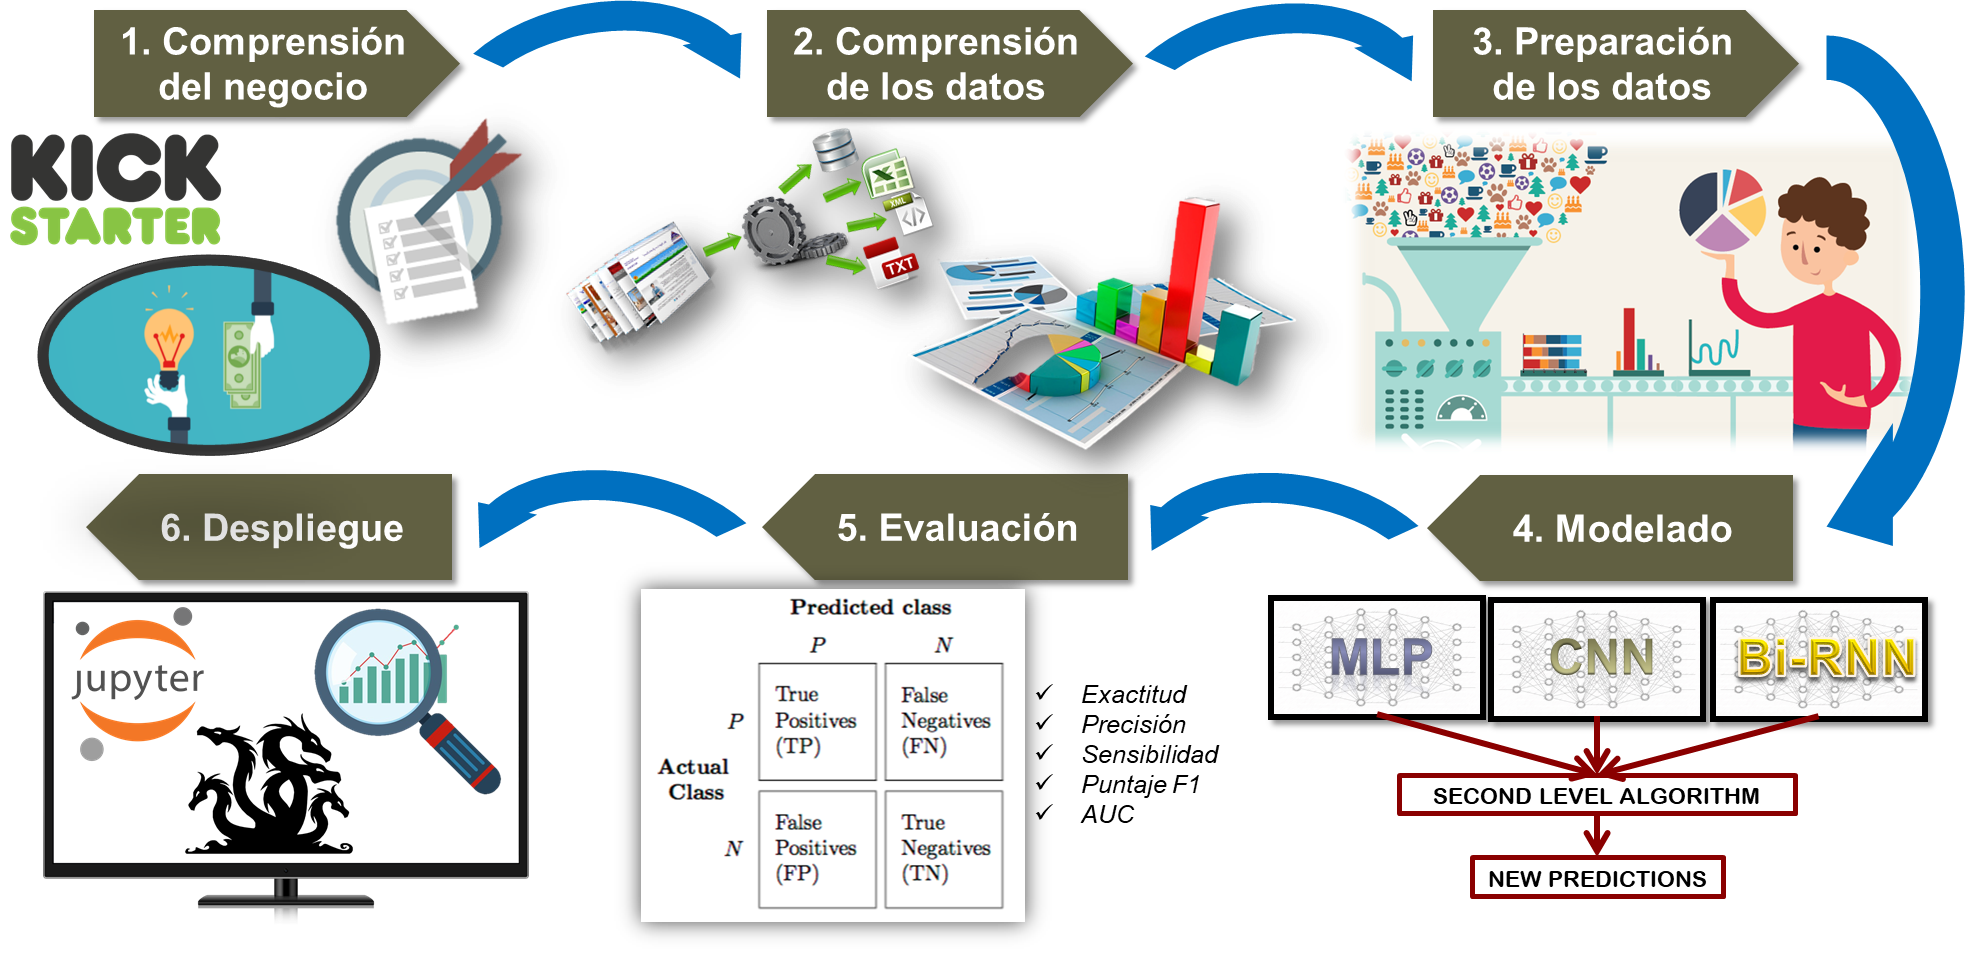
\includegraphics[width=1\textwidth]{3/figures/metodologia.png}
		\caption[Metodología de la investigación]{Metodología de la investigación.\\
			Fuente: Elaboración propia}
		\label{3:fig2}
	\end{center}
\end{figure}

A continuación, se explicarán las actividades y tareas efectuadas a lo largo de su implementación.

\subsubsection{Comprensión del negocio}
En la primera fase, se definió el problema a partir de comprender el contexto de la investigación. A partir de aquí, se formularon los objetivos y requerimientos que se espera lograr en el proyecto. La lista de actividades y tareas se presenta en la Tabla \ref{3:table3}.

%\begingroup
%\renewcommand\arraystretch{0.3}
\begin{longtable}{|M{5cm}|M{5cm}|M{5cm}|}
	\caption[Actividades de fase Comprensión del negocio]{Actividades de fase Comprensión del negocio.}
	\label{3:table3}
	\newcommand{\multirot}[1]{\multirow{2}{*}[-8ex]{\rotcell{\rlap{#1}}}}
	%\scriptsize
	\footnotesize
	\centering
	\small
	%% Se agrega tabularnewline para longtable
	\tabularnewline\hline
	\textbf{Actividades} & \textbf{Descripción} & \textbf{Tareas}
	\\
	\hline
	a
	& 1
	& 6                                               
	\\
	\hline
	b
	& 2
	& 6
	\\
	\hline
	c
	& 1
	& 6
	\\
	\hline
	d
	& 2
	& 5
	\\
	\hline
	e
	& 3
	& 5
	\\
	\hline
	f
	& 3
	& 5
	\\
	\hline
	g
	& 3
	& 4
	\\
	\hline
	h
	& 1
	& 4
	\\
	\hline
	i
	& 2
	& 3
	\\
	\hline
\end{longtable}%
%\endgroup

%\par	%%Salto de linea
%\bigskip
\begin{flushleft}	%%Alinear a la izquierda sin justificar
	\small Fuente: Elaboración propia
\end{flushleft}

Para empezar, el crowdfunding se basa, como su nombre en inglés lo indica, en lograr que un proyecto emprendedor sea llevado a cabo gracias al financiamiento colectivo. Existen 4 diferentes modelos de crowdfunding: basado en donaciones, basado en recompensas, basado en capital social y basado en deuda. El crowdfunding basado en capital social se encuentra actualmente limitado en los Estados Unidos debido a que la Regulación D de la Ley de Valores de 1933 prohíbe la participación de muchos potenciales inversionistas y los obliga a tener un ingreso anual mayor a \$200,000 o más de \$1 millón en patrimonio neto \parencite{cr_lichtig2015crowdfunding}.

El modelo basado en donaciones se refiere a la recaudación de fondos a través de la Web 2.0, en el cual los patrocinadores no esperan recompensas materiales a cambio sino más bien una recompensa social. Por el contrario, el modelo basado en recompensas ofrece compensación tanto material como inmaterial y representa hoy en día el modelo de crowdfunding más frecuente. Los financiadores, por un lado, pueden verse beneficiados de la venta anticipada, recibiendo el proyecto o producto financiado antes de su publicación o entrada al mercado al mejor precio. Los proyectos que pertenecen a esta categoría a menudo son organizaciones sin fines de lucro \parencite{cr_kraus2016crowdfunding_strategies}.

Kickstarter, la plataforma de crowdfunding más citada, analizada y una de las más grandes, es una comunidad basada en el crowdfunding por recompensas. A la fecha, 128 mil proyectos han sido financiados, 3 billones de dólares fueron prometidos en proyectos y 13 millones de patrocinadores han participado, del cual el 31\% ha colocado dinero en más de 1 proyecto.

La particularidad de los proyectos en esta plataforma es que, luego de cumplir un plazo de tiempo determinado, el monto prometido acumulado puede ser asignado a los proyectos que hayan alcanzado o superado la meta estipulada al inicio. Para ello, los dueños de los proyectos tienen que crear estrategias para lograr campañas exitosas y hacer realidad su producto. Un 75\% de los proyectos que fueron apoyados por al menos 25 patrocinadores han sido financiados exitosamente \parencite{cr_kickstarter_learn}.

Para lograr que un proyecto en la plataforma logre impactar en la comunidad, debe contar con conexiones duraderas, retroalimentación del producto y ser tangible. Asimismo, algunos enfoques importantes se basan en probar nuevas ideas, aumentar la comunidad y cubrir costos de manufacturación.

Para empezar a realizar la campaña del proyecto, es necesario seguir las sugerencias basadas en los autores \cite{cr_yu2017kickstarter_course} y \cite{cr_kickstarter_intro}:
\begin{itemize}
	\item Identificar la meta óptima del proyecto. Se debe realizar una lista de todos los costos, así como el shipping que deben de cada país. También se debe contar con un buffer en caso ocurra un imprevisto. Se puede determinar la meta a través de la fórmula (Gastos + Buffer) x Alcance.
	\item Crear el video de la campaña en un presupuesto. El vídeo resulta ser un factor muy importante ya que aquellos que cuentan con un video de su proyecto tienen un 50\% de chance de tener éxito. El promedio debería ser de 3.38 minutos, aunque el público presta más atención hacia aquellos que duran poco. El vídeo debe contener y responder las siguientes preguntas:
	\begin{itemize}
		\item ¿Qué hace memorable al proyecto?
		\item ¿Cómo se verá el proyecto?
		\item ¿Por qué se está creando el producto?
		\item ¿Por qué lo necesitas?
		\item ¿Por qué es importante que tu proyecto exista?
		\item ¿Por qué debes ser tú su creador?
		\item ¿Por qué tu compañía?
		\item ¿Cómo proveerás una solución?
		\item ¿Cómo funciona la solución?
	\end{itemize}
	Es importante destacar las estadísticas del problema que se piensa resolver al inicio del video ya que el primer minuto resulta ser el lapso de tiempo que más capta la atención del público. Se recomienda también tener buen audio e iluminación.
	\item Escribir la descripción del proyecto. Otro factor clave en el desempeño de la campaña de un proyecto en Kickstarter resulta ser la descripción que representa un resumen de los puntos más relevantes del producto. Se debe mencionar una breve introducción del proyecto, cómo funciona, para quiénes son, el proceso que se siguió en el desarrollo, detalles y especificaciones, y un cronograma e hitos.
	\item Incluir imágenes sobre cómo lucirá el proyecto. Esta prueba convencerá a más de una persona en querer invertir en el proyecto. Las imágenes a veces atraen más a las personas que no gustan leer la descripción completa del proyecto.
	\item Determinar las recompensas del proyecto. Al basarse en un modelo de crowdfunding en recompensas, los patrocinadores esperan un beneficio por parte del proyecto una vez este logre alcanzar su financiamiento. El número ideal de recompensas puede ser entre 5 y 7. Una recompensa en promedio de \$100 es la que genera más dinero. Las recompensas pueden ser de cuatro tipos: el producto en sí mismo entregado hacia los patrocinadores antes que este salga al mercado, reconocimientos en la página web y acceso hacia actualizaciones, recuerdos y certificados de membresía, y nuevas experiencias como visita a los desarrolladores en sus estudios.
\end{itemize}

Todos los factores anteriormente mencionados determinarán en gran medida el nivel de éxito que tendrá un proyecto una vez su campaña sea lanzada en la plataforma.

\subsubsection{Comprensión de los datos}
La segunda fase abarcó tanto la recolección de los datos como el análisis estadístico de estos para conocer un poco más sus características. El conjunto total de datos utilizado para la investigación consistió en la recolección de 27,251 proyectos tecnológicos de Kickstarter comprendidos entre los años 2009 y 2019, en 3 partes: metainformación, descripción y comentarios (excluyendo los del creador) del proyectos.

Para ello, se elaboró una lista de actividades y tareas presentadas en la Tabla \ref{3:table4}.

%\begingroup
%\renewcommand\arraystretch{0.5}
\begin{longtable}{|M{4cm}|M{5.5cm}|M{5.5cm}|}
	\caption[Actividades de fase Comprensión de los datos]{Actividades de fase Comprensión de los datos.}
	\label{3:table4}
	\newcommand{\multirot}[1]{\multirow{2}{*}[-8ex]{\rotcell{\rlap{#1}}}}
	%\scriptsize
	\footnotesize
	\centering
	\small
	%% Se agrega tabularnewline para longtable
	\tabularnewline\hline
	\textbf{Actividades} & \textbf{Descripción} & \textbf{Tareas}
	\\
	\hline
	Construir base de datos de Metainformación.
	& Construcción de base de datos que contenga las variables de la campaña con excepción del contenido textual (descripción, actualizaciones y comentarios acerca del proyecto).
	& \setlist{nolistsep}
	\begin{itemize}[noitemsep,leftmargin=*]
		\item Descargar conjuntos de datos comprimidos de la página Web Robots.
		\item Descomprimir archivos en partes y fusionarlos en uno solo según su mes.
		\item Fusionar archivos por mes, realizar limpieza de datos y generar base final.
	\end{itemize} 
	\\
	\hline
	Construir base de datos de Descripción.
	& Construcción de base de datos que contenga la descripción del proyecto en la página principal de la campaña.
	& \setlist{nolistsep}
	\begin{itemize}[noitemsep,leftmargin=*]
		\item Identificar sección de descripción a partir de la búsqueda del URL desde la base de datos de Metainformación.
		\item Capturar información de sección identificada.
		\item Generar base final.
	\end{itemize} 
	\\
	\hline
	Construir base de datos de Comentarios.
	& Construcción de base de datos que contenga los comentarios de los patrocinadores del proyecto en su sección correspondiente.
	& \setlist{nolistsep}
	\begin{itemize}[noitemsep,leftmargin=*]
		\item Identificar sección de comentarios a partir de la búsqueda del URL desde la base de datos de Metainformación.
		\item Capturar información de sección identificada, excluyendo comentarios y respuestas de los creadores del proyecto.
		\item Generar base final.
	\end{itemize}
	\\
	\hline
	Realizar análisis exploratorio y estadístico de variables considerados.
	& Análisis exploratorio y estadístico de las variables disponibles para cada modalidad.
	& \setlist{nolistsep}
	\begin{itemize}[noitemsep,leftmargin=*]
		\item Describir distribución de los datos y tendencias.
		\item Analizar existencia de correlación en caso se encuentre presente.
	\end{itemize}
	\\
	\hline
\end{longtable}%
%\endgroup

%\par	%%Salto de linea
%\bigskip
\begin{flushleft}	%%Alinear a la izquierda sin justificar
	\small Fuente: Elaboración propia
\end{flushleft}

A continuación, cada actividad de la anterior tabla es detallada y se indican sus entregables respectivos.

\textbf{Actividad 1: Construir base de datos de Metainformación}
\\
De acuerdo a la Figura \ref{3:fig1}, en esta actividad se enfocó en la construcción de la base de datos de la Metainformación desde la descarga de los conjuntos de datos comprimidos de la página Web Robots hasta la generación del archivo final luego de limpiar los datos.

La 2 primeras tareas de la anterior tabla se resumen en el flujo de la Figura \ref{3:fig3}.

\begin{figure}[h]
	\begin{center}
		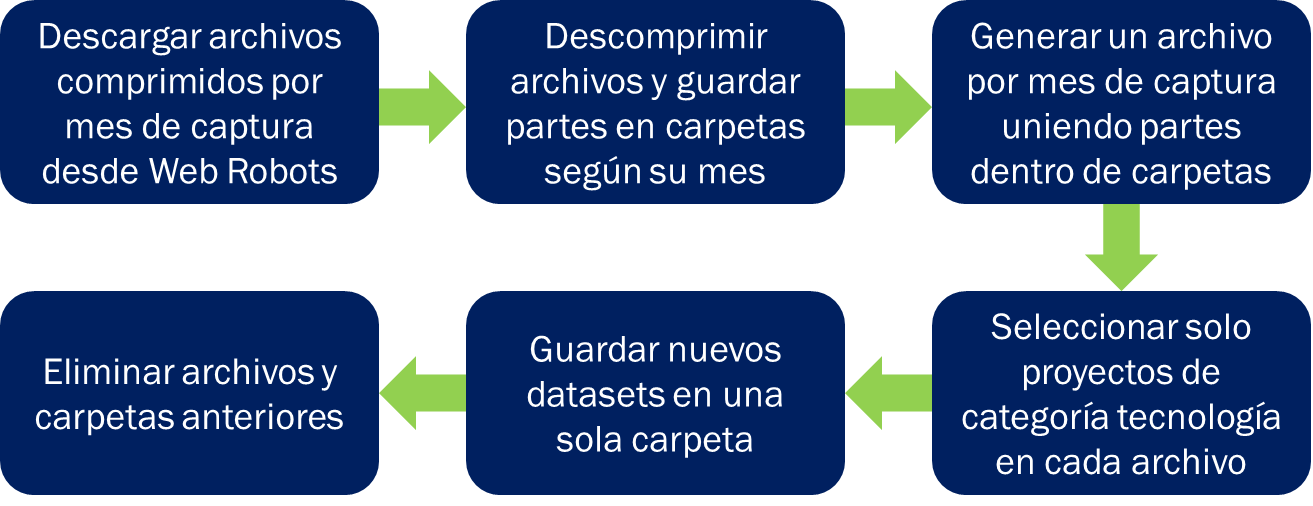
\includegraphics[width=0.8\textwidth]{3/figures/flujograma_metadata_t1_t2.png}
		\caption[Proceso de obtención y preparación de datasets iniciales de Metainformación]{Proceso de obtención y preparación de datasets iniciales de Metainformación.\\
			Fuente: Elaboración propia.}
		\label{3:fig3}
	\end{center}
\end{figure}

La siguiente fase de la actividad fue la selección de variables y limpieza de datos utilizando el software Alteryx Designer, el cual permite desarrollar flujos de trabajo para preparar, unir y analizar volúmenes de datos complejos de distintas fuentes. Se ejecutó el flujograma representado de forma resumida en la Figura \ref{3:fig4}.

\begin{figure}[h]
	\begin{center}
		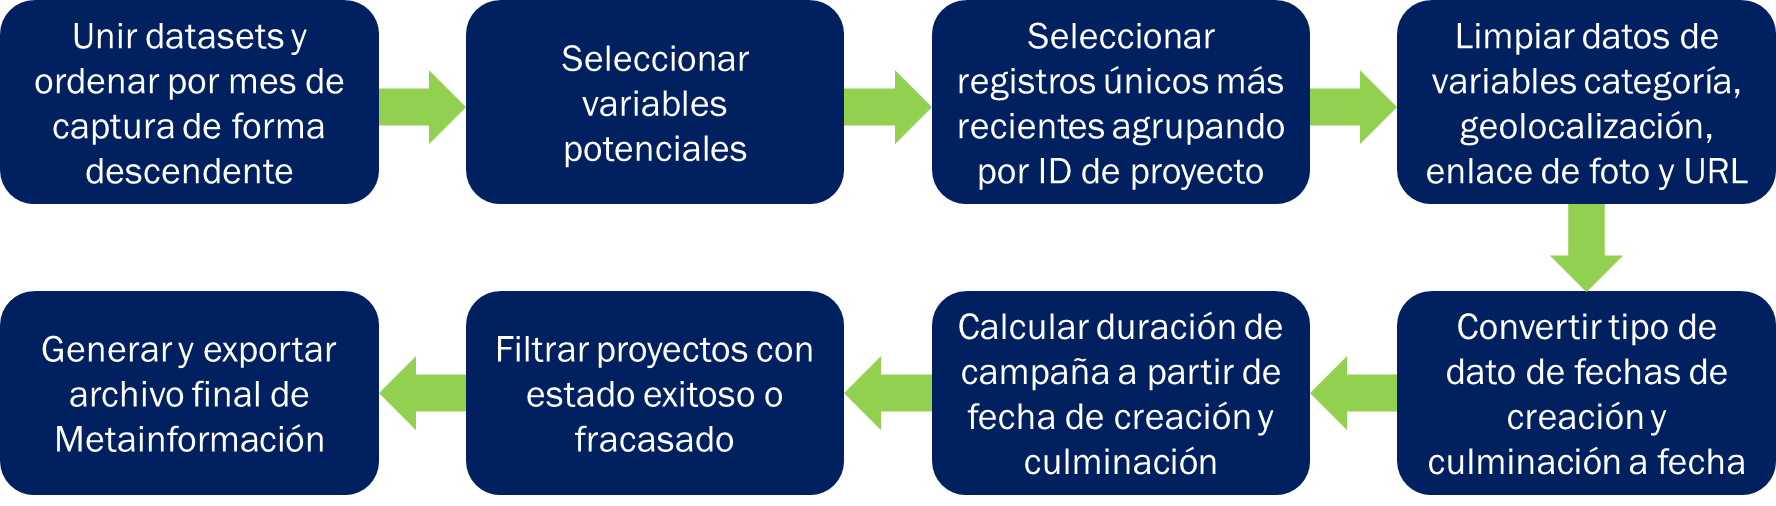
\includegraphics[width=1\textwidth]{3/figures/flujograma_metadata_t3.png}
		\caption[Proceso resumido de generación de conjunto final de Metainformación]{Proceso resumido de generación de conjunto final de Metainformación.\\
			Fuente: Elaboración propia.}
		\label{3:fig4}
	\end{center}
\end{figure}

\textbf{Entregable}: Conjunto de datos de Metainformación, que contiene 19 variables cuantitativas y cualitativas para la muestra considerada.

\textbf{Actividad 2: Construir base de datos de Descripción}
\\
De acuerdo a la Figura \ref{3:fig1}, una vez generado el conjunto de datos de Metainformación descrito en la anterior actividad, a partir de la variable \textit{urls} se puede extraer la descripción de cada proyecto, siguiendo el proceso del diagrama de flujo representado en la Figura \ref{3:fig5}.

\begin{figure}[h]
	\begin{center}
		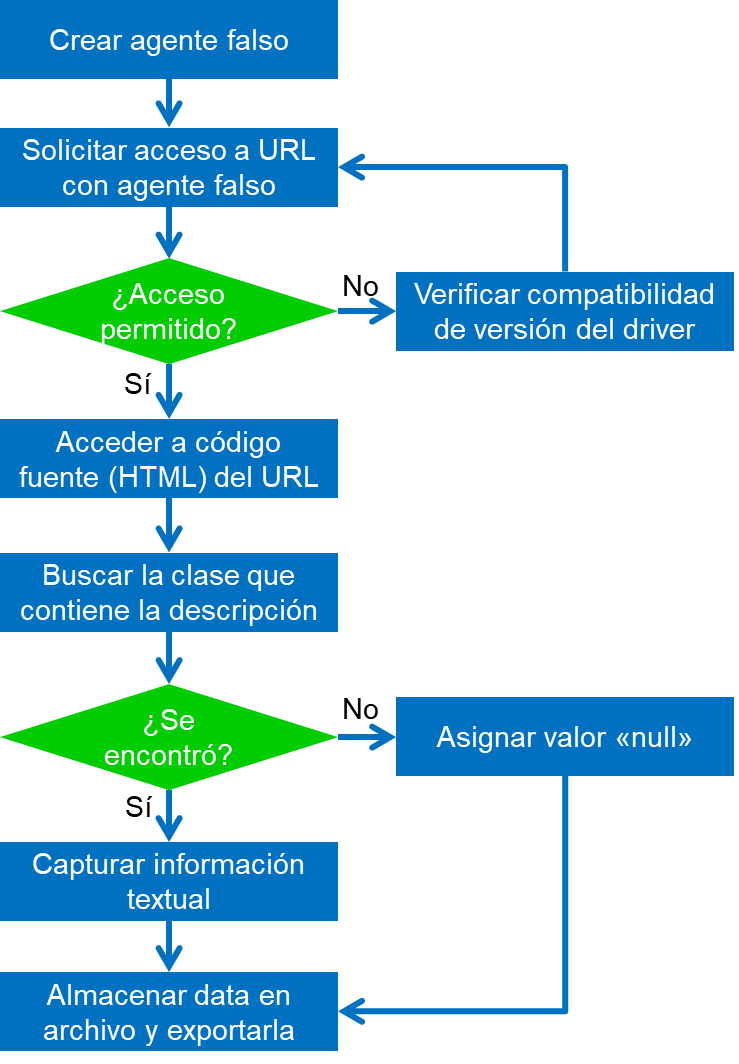
\includegraphics[width=0.5\textwidth]{3/figures/diagrama_flujo_scrapping_descripcion.png}
		\caption[Diagrama de flujo del proceso de extracción de la descripción de un proyecto]{Diagrama de flujo del proceso de extracción de la descripción de un proyecto.\\
			Fuente: Elaboración propia.}
		\label{3:fig5}
	\end{center}
\end{figure}

\textbf{Entregable}: Conjunto de datos de Descripción, que contiene la variable textual de descripción del proyecto para la muestra considerada.

\textbf{Actividad 3: Construir base de datos de Comentarios}
\\
De acuerdo a la Figura \ref{3:fig1}, y realizando el mismo ejercicio con Descripción, una vez generado el conjunto de datos de Metainformación, a partir de la variable \textit{urls} se pueden extraer los comentarios de los patrocinadores por cada proyecto, siguiendo el proceso del diagrama de flujo representado en la Figura \ref{3:fig6}.

\begin{figure}[h]
	\begin{center}
		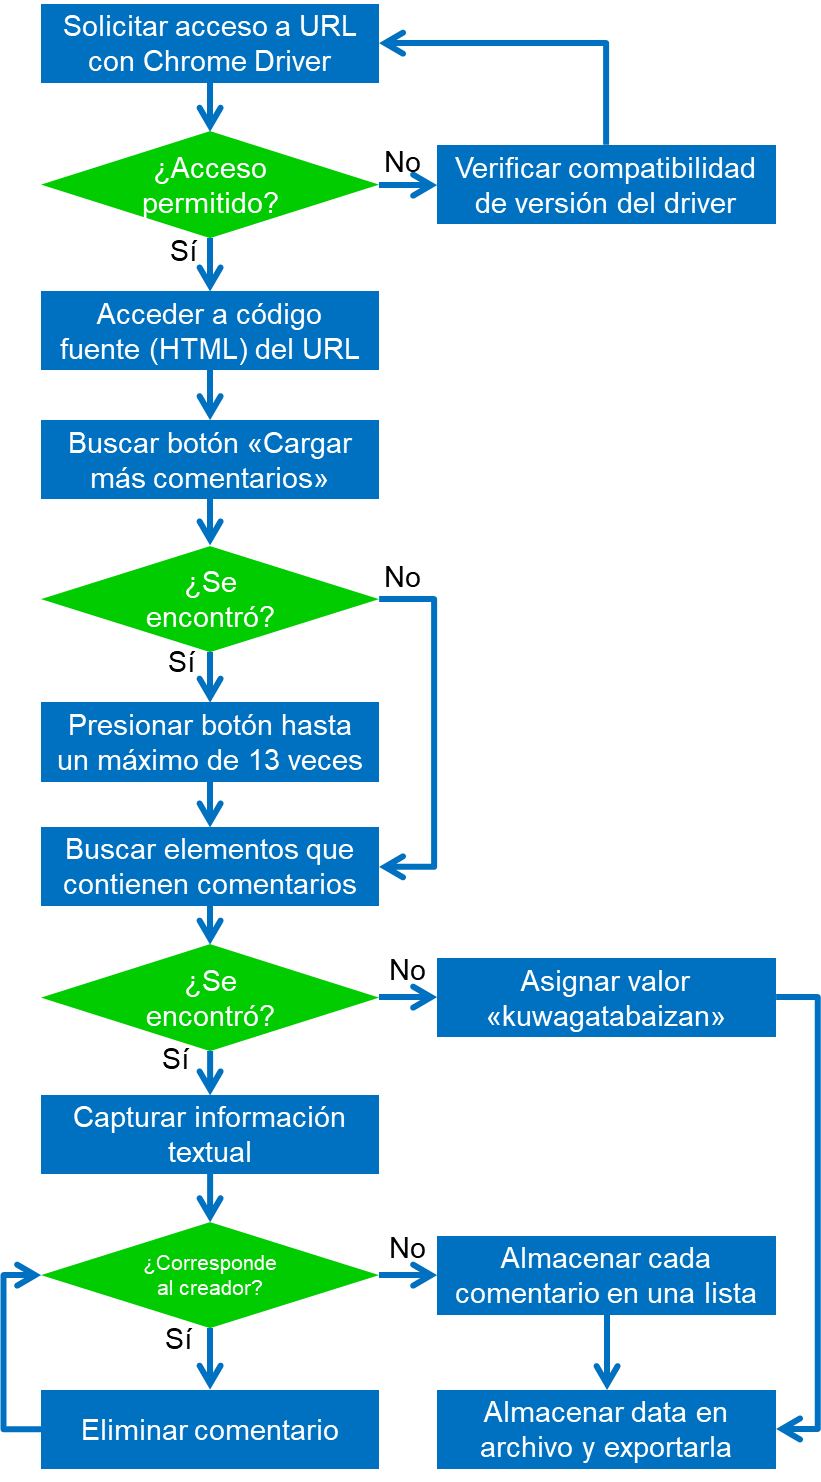
\includegraphics[width=0.45\textwidth]{3/figures/diagrama_flujo_scrapping_comentarios.png}
		\caption[Diagrama de flujo del proceso de extracción de comentarios de un proyecto]{Diagrama de flujo del proceso de extracción de comentarios de un proyecto.\\
			Fuente: Elaboración propia.}
		\label{3:fig6}
	\end{center}
\end{figure}

\textbf{Entregable}: Conjunto de datos de Comentarios, que contiene la variable textual de comentarios de los patrocinadores, cada uno separado por autor y almacenados en conjunto en una lista por proyecto, para la muestra considerada.

\textbf{Actividad 4: Realizar análisis exploratorio y estadístico de variables considerados}
\\

\textbf{Entregable}:

\subsubsection{Preparación de los datos}
El análisis exploratorio de los datos fue determinante para la selección final de variables de la Metainformación, gracias al uso de herramientas estadísticas como el análisis de correlaciones para discriminar aquellas que superaron el límite fijado y que desembocó, luego del pre-procesamiento detallado en el subcapítulo 3 del mismo capítulo, en la Tabla \ref{3:table5}.

%\begingroup
%\renewcommand\arraystretch{0.3}
\begin{longtable}{|M{5cm}|M{5cm}|M{5cm}|}
	\caption[Actividades de fase Preparación de los datos]{Actividades de fase Preparación de los datos.}
	\label{3:table5}
	\newcommand{\multirot}[1]{\multirow{2}{*}[-8ex]{\rotcell{\rlap{#1}}}}
	%\scriptsize
	\footnotesize
	\centering
	\small
	%% Se agrega tabularnewline para longtable
	\tabularnewline\hline
	\textbf{Actividades} & \textbf{Descripción} & \textbf{Tareas}
	\\
	\hline
	Pre-procesar base de datos de Metainformación.
	& Pre-procesamiento de las variables actuales y adicionales luego de evaluación de su comportamiento entre ellas.
	& \setlist{nolistsep}
	\begin{itemize}[noitemsep,leftmargin=*]
		\item Añadir más variables cuantitativas según literatura.
		\item Evaluar comportamiento de variables en conjunto utilizando matriz de correlaciones.
		\item Armar grupos combinatorias potenciales de variables.
		\item Escalar variables a un mismo rango.
	\end{itemize}                                             
	\\
	\hline
	Pre-procesar base de datos de Descripción.
	& Pre-procesamiento de la variable \textit{description}.
	& \setlist{nolistsep}
	\begin{itemize}[noitemsep,leftmargin=*]
		\item Realizar limpieza de datos de los textos.
		\item Armar vocabulario de palabras únicas.
		\item Transformar textos en vectores de palabras.
	\end{itemize} 
	\\
	\hline
	Pre-procesar base de datos de Comentarios.
	& Pre-procesamiento de la variable \textit{comments}.
	& \setlist{nolistsep}
	\begin{itemize}[noitemsep,leftmargin=*]
		\item Realizar limpieza de datos de los textos.
		\item Armar vocabulario de palabras únicas.
		\item Transformar textos en vectores de palabras.
	\end{itemize}
	\\
	\hline
\end{longtable}%
%\endgroup

%\par	%%Salto de linea
%\bigskip
\begin{flushleft}	%%Alinear a la izquierda sin justificar
	\small Fuente: Elaboración propia
\end{flushleft}

\subsubsection{Modelamiento}



%\begingroup
%\renewcommand\arraystretch{0.3}
\begin{longtable}{|M{5cm}|M{5cm}|M{5cm}|}
	\caption[Actividades de fase Modelamiento]{Actividades de fase Modelamiento.}
	\label{3:table6}
	\newcommand{\multirot}[1]{\multirow{2}{*}[-8ex]{\rotcell{\rlap{#1}}}}
	%\scriptsize
	\footnotesize
	\centering
	\small
	%% Se agrega tabularnewline para longtable
	\tabularnewline\hline
	\textbf{Actividades} & \textbf{Descripción} & \textbf{Tareas}
	\\
	\hline
	Desarrollar modelo predictivo de Metainformación.
	& Implementación del modelo Perceptrón Multicapa (MLP) para la modalidad Metainformación.
	& \setlist{nolistsep}
	\begin{itemize}[noitemsep,leftmargin=*]
		\item Diseñar arquitectura del modelo predictivo.
		\item Entrenar cada grupo de combinatoria de variables con arquitectura diseñada.
		\item Realizar experimentos con hiperparámetros modificados.
		\item Comparar desempeños individuales entre todos los grupos.
	\end{itemize}
	\\
	\hline
	Desarrollar modelo predictivo de Descripción.
	& Implementación de la Red Neuronal Convolucional (CNN) para la modalidad Descripción.
	& \setlist{nolistsep}
	\begin{itemize}[noitemsep,leftmargin=*]
		\item Diseñar arquitectura del modelo predictivo.
		\item Entrenar base de datos pre-procesada con arquitectura diseñada.
		\item Realizar experimentos con hiperparámetros modificados.
		\item Comparar resultados obtenidos.
	\end{itemize}
	\\
	\hline
	Desarrollar modelo predictivo de Comentarios.
	& Implementación del modelo LSTM Bidireccional para la modalidad Comentarios.
	& \setlist{nolistsep}
	\begin{itemize}[noitemsep,leftmargin=*]
		\item Diseñar arquitectura del modelo predictivo.
		\item Entrenar base de datos pre-procesada con arquitectura diseñada.
		\item Realizar experimentos con hiperparámetros modificados.
		\item Comparar resultados obtenidos.
	\end{itemize}
	\\
	\hline
\end{longtable}%
%\endgroup

%\par	%%Salto de linea
%\bigskip
\begin{flushleft}	%%Alinear a la izquierda sin justificar
	\small Fuente: Elaboración propia
\end{flushleft}

Luego del pre-procesamiento de los datos, en esta fase se procedió a crear modelos predictivos para cada modalidad considerada. Tomando de referencia a los antecedentes del Marco Teórico, los más usados para cada modalidad se detalla a continuación:
\begin{itemize}
	\item \textbf{Metainformación}: Perceptrón Multicapa (\cite{pr_kamath2018suplearn}; \cite{pr_yu2018deeplearning}; \cite{pr_cheng2019deeplearning}), Máquina de Vectores de Soporte (\cite{pr_chen2013kickpredict}; \cite{pr_beckwith2016predcrowd}; \cite{pr_sawhney2016usingLT}), Regresión Logística (\cite{pr_mitra2014phrases}; \cite{pr_zhou2015projectdesc}; \cite{pr_beckwith2016predcrowd}; \cite{pr_li2016predcrowd}; \cite{pr_kaur2017socmedcrowd}), Regresión Log-logística (\cite{pr_li2016predcrowd}), Bosques Aleatorios (\cite{pr_chen2015predcrowd}; \cite{pr_yuan2016textanalytics}; \cite{pr_kamath2018suplearn}), Árboles de Decisión (\cite{pr_beckwith2016predcrowd}; \cite{pr_kamath2018suplearn}), Naïve Bayes (\cite{pr_beckwith2016predcrowd}; \cite{pr_kamath2018suplearn}), Modelo Seq2seq (\cite{pr_jin2019dayssuccess}).
	\item \textbf{Descripción}: CNN (\cite{pr_cheng2019deeplearning}), LSTM (\cite{pr_jin2019dayssuccess}), Modelo Seq2seq (\cite{pr_lee2018contentDL}), Máquina de Vectores de Soporte o variantes (\cite{pr_sawhney2016usingLT}; \cite{pr_chen2019keywords_crowdfunding}), Regresión Logística (\cite{pr_mitra2014phrases}; \cite{pr_zhou2015projectdesc}), LDA o variantes (\cite{pr_yuan2016textanalytics}; \cite{pr_sawhney2016usingLT}).
	\item \textbf{Comentarios}: LSTM (\cite{pr_jin2019dayssuccess}; \cite{pr_shafqat2019topicpredictions}), LDA o variantes (\cite{pr_shafqat2019topicpredictions}), Modelo Seq2seq (\cite{pr_lee2018contentDL}; \cite{pr_jin2019dayssuccess}), HAN (\citeauthor{pr_lee2018contentDL}), Regresión Logística (\cite{pr_li2016predcrowd}; \cite{pr_kaur2017socmedcrowd}), Regresión Log-logística (\cite{pr_li2016predcrowd}).
\end{itemize}

De todos los modelos mencionados, los más predominantes de Aprendizaje Automático fueron las Máquinas de Vectores de Soporte y los de Regresión Logística, mientras que por el lado de Aprendizaje Profundo, fueron los Perceptrones Multicapa aunque las otras redes enunciadas derivan de este tipo.

Según los anteriores autores, salvo en investigaciones donde se usaron 1 sola modalidad, como por ejemplo la Metainformación, los modelos de Aprendizaje Profundo tuvieron mejor desempeño que los tradicionales de Aprendizaje Automático. Además, dado que la propuesta de esta investigación es ensamblar múltiples modelos, considerar un mix de ambos tipos de arquitectura resulta inviable por la complejidad de transformación de sus salidas de distintos tamaños.

Por ello, se optó por usar arquitecturas de Redes Neuronales para cada modalidad con el fin de poder ensamblar y comparar sus resultados, tanto de manera individual como en el modelo apilado, con la literatura.

Teniendo como referencia investigaciones basadas en Aprendizaje Profundo Multimodal, es decir, que combinan distintas características de una campaña de crowdfunding (\cite{pr_kamath2018suplearn}, décimo antecedente; \cite{pr_jin2019dayssuccess}, decimotercer antecedente; \cite{pr_cheng2019deeplearning}, decimocuarto antecedente) usando Metainformación (\cite{pr_chen2013kickpredict}, primer antecedente; \cite{pr_mitra2014phrases}, segundo antecedente; \cite{pr_zhou2015projectdesc}, tercer antecedente; \cite{pr_chen2015predcrowd}, cuarto antecedente; \cite{pr_beckwith2016predcrowd}, quinto antecedente; \cite{pr_li2016predcrowd}, sexto antecedente; \cite{pr_yuan2016textanalytics}, séptimo antecedente; \cite{pr_sawhney2016usingLT}, octavo antecedente; \cite{pr_kaur2017socmedcrowd}, noveno antecedente; \cite{pr_kamath2018suplearn}, décimo antecedente; \cite{pr_yu2018deeplearning}, undécimo antecedente; \cite{pr_jin2019dayssuccess}, decimotercer antecedente; \cite{pr_cheng2019deeplearning}, decimocuarto antecedente), descripción del proyecto (\cite{pr_mitra2014phrases}, segundo antecedente; \cite{pr_zhou2015projectdesc}, tercer antecedente; \cite{pr_yuan2016textanalytics}, séptimo antecedente; \cite{pr_sawhney2016usingLT}, octavo antecedente; \cite{pr_lee2018contentDL}, duodécimo antecedente; \cite{pr_jin2019dayssuccess}, decimotercer antecedente; \cite{pr_cheng2019deeplearning}, decimocuarto antecedente; \cite{pr_chen2019keywords_crowdfunding}, decimoquinto antecedente; \cite{pr_chaichi2019nlp_3dprinting}, decimosexto antecedente) y comentarios de los patrocinadores acerca del mismo (\cite{pr_chen2015predcrowd}, cuarto antecedente; \cite{pr_li2016predcrowd}, sexto antecedente; \cite{pr_lee2018contentDL}, duodécimo antecedente; \cite{pr_jin2019dayssuccess}, decimotercer antecedente; \cite{pr_shafqat2019topicpredictions}, decimoséptimo antecedente), la idea del prototipo final consistió en ensamblar estas 3 partes en un modelo apilado. Para ello, se representa cada una de las tres partes agrupadas en el marco de trabajo de la Figura \ref{3:fig7}.
\begin{figure}[htbp]
	\begin{center}
		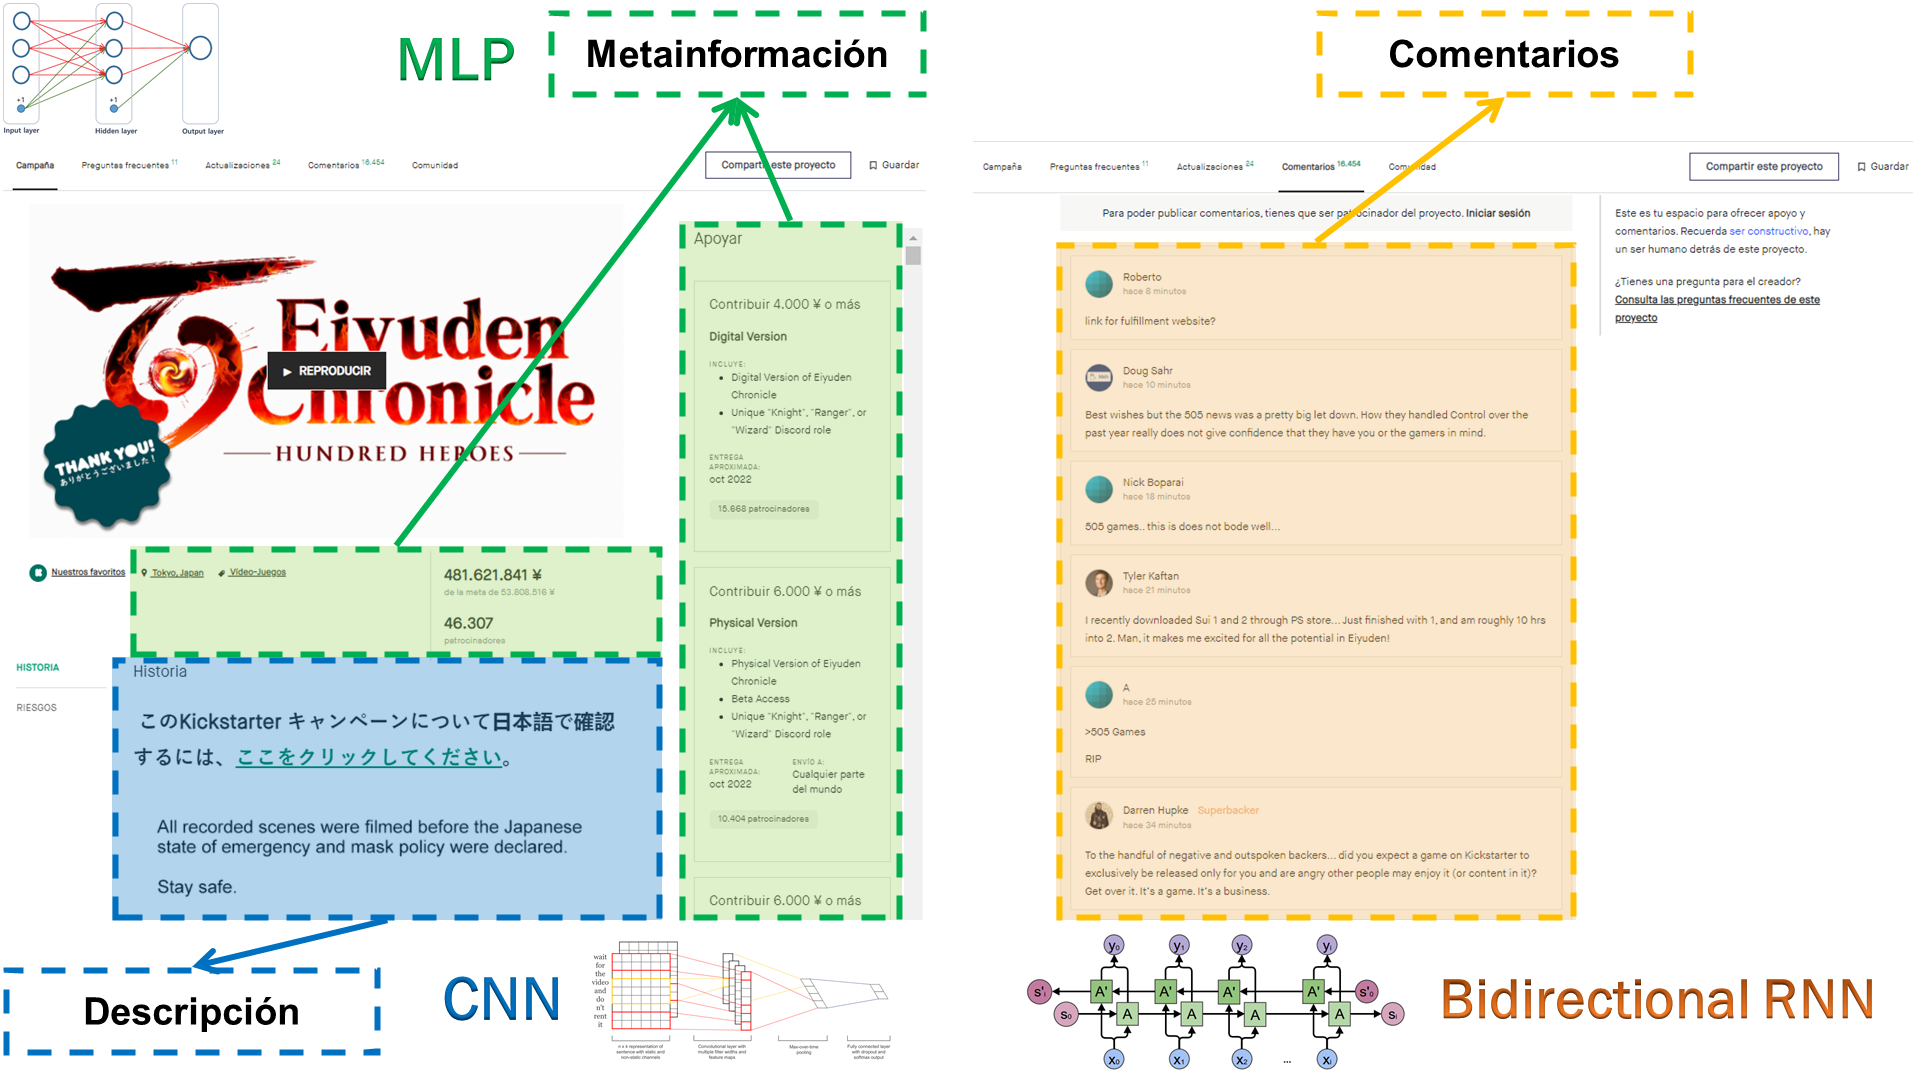
\includegraphics[width=1\textwidth]{3/figures/framework.png}
		\caption[Marco de trabajo del prototipo final]{Marco de trabajo del prototipo final.\\
			Fuente: Elaboración propia}
		\label{3:fig7}
	\end{center}
\end{figure}

\subsubsection{Evaluación}

%\begingroup
%\renewcommand\arraystretch{0.3}
\begin{longtable}{|M{5cm}|M{5cm}|M{5cm}|}
	\caption[Actividades de fase Evaluación]{Actividades de fase Evaluación.}
	\label{3:table7}
	\newcommand{\multirot}[1]{\multirow{2}{*}[-8ex]{\rotcell{\rlap{#1}}}}
	%\scriptsize
	\footnotesize
	\centering
	\small
	%% Se agrega tabularnewline para longtable
	\tabularnewline\hline
	\textbf{Actividades} & \textbf{Descripción} & \textbf{Tareas}
	\\
	\hline
	a
	& 1
	& 6                                               
	\\
	\hline
	b
	& 2
	& 6
	\\
	\hline
	c
	& 1
	& 6
	\\
	\hline
	d
	& 2
	& 5
	\\
	\hline
	e
	& 3
	& 5
	\\
	\hline
	f
	& 3
	& 5
	\\
	\hline
	g
	& 3
	& 4
	\\
	\hline
	h
	& 1
	& 4
	\\
	\hline
	i
	& 2
	& 3
	\\
	\hline
\end{longtable}%
%\endgroup

%\par	%%Salto de linea
%\bigskip
\begin{flushleft}	%%Alinear a la izquierda sin justificar
	\small Fuente: Elaboración propia
\end{flushleft}


De las métricas de clasificación de Aprendizaje Automático explicadas en el cuarto subcapítulo del presente capítulo, las usadas por los autores de la literatura fueron las siguientes:

\begin{itemize}
	\item \textbf{Exactitud}: \cite{pr_chen2013kickpredict}, \cite{pr_chen2015predcrowd}, \cite{pr_beckwith2016predcrowd}, \cite{pr_yuan2016textanalytics}, \cite{pr_sawhney2016usingLT}, \cite{pr_kaur2017socmedcrowd}, \cite{pr_kamath2018suplearn}, \cite{pr_yu2018deeplearning}, \cite{pr_lee2018contentDL}, \cite{pr_cheng2019deeplearning}, \cite{pr_chen2019keywords_crowdfunding}, \cite{pr_shafqat2019topicpredictions}.
	\item \textbf{Precisión}: \cite{pr_beckwith2016predcrowd}, \cite{pr_yuan2016textanalytics}, \cite{pr_kaur2017socmedcrowd}, \cite{pr_cheng2019deeplearning}.
	\item \textbf{Sensibilidad}: \cite{pr_beckwith2016predcrowd}, \cite{pr_yuan2016textanalytics}, \cite{pr_kaur2017socmedcrowd}, \cite{pr_cheng2019deeplearning}, \cite{pr_chen2019keywords_crowdfunding}.
	\item \textbf{Especificidad}: \cite{pr_chen2019keywords_crowdfunding}.
	\item \textbf{Ratio de Falsa Alarma}: \cite{pr_kaur2017socmedcrowd}.
	\item \textbf{Media Geométrica (G-Mean)}: \cite{pr_chen2019keywords_crowdfunding}.
	\item \textbf{Puntaje F1}: \cite{pr_zhou2015projectdesc}, \cite{pr_beckwith2016predcrowd}, \cite{pr_yuan2016textanalytics}, \cite{pr_kaur2017socmedcrowd}, \cite{pr_cheng2019deeplearning}, \cite{pr_chen2019keywords_crowdfunding}.
	\item \textbf{Curva ROC}: \cite{pr_zhou2015projectdesc}, \cite{pr_beckwith2016predcrowd}.
	\item \textbf{Área bajo la Curva ROC (AUC)}: \cite{pr_beckwith2016predcrowd}, \cite{pr_li2016predcrowd}, \cite{pr_kaur2017socmedcrowd}, \cite{pr_yu2018deeplearning}, \cite{pr_cheng2019deeplearning}.
	\item \textbf{Área bajo la Curva Precisión-Sensibilidad (PRC)}: \cite{pr_kaur2017socmedcrowd}.
	\item \textbf{Error de Validación Cruzada}: \cite{pr_mitra2014phrases}.
	\item \textbf{Coeficiente de Correlación de Matthew (MCC)}: \cite{pr_kaur2017socmedcrowd}.
	\item \textbf{Divergencia de Kullback-Leibler (KL)}: \cite{pr_jin2019dayssuccess}.
	\item \textbf{Raíz del Error Cuadrático Medio (RMSE)}: \cite{pr_jin2019dayssuccess}.
	\item \textbf{Error Absoluto Medio (MAE)}: \cite{pr_jin2019dayssuccess}.
	\item \textbf{Índice de Concordancia (CI)}: \cite{pr_jin2019dayssuccess}.
\end{itemize}

En el Capítulo 5 se explica cuáles fueron seleccionadas para evaluar cada modelo.

\subsubsection{Despliegue}

%\begingroup
%\renewcommand\arraystretch{0.3}
\begin{longtable}{|M{5cm}|M{5cm}|M{5cm}|}
	\caption[Actividades de fase Despliegue]{Actividades de fase Despliegue.}
	\label{3:table8}
	\newcommand{\multirot}[1]{\multirow{2}{*}[-8ex]{\rotcell{\rlap{#1}}}}
	%\scriptsize
	\footnotesize
	\centering
	\small
	%% Se agrega tabularnewline para longtable
	\tabularnewline\hline
	\textbf{Actividades} & \textbf{Descripción} & \textbf{Tareas}
	\\
	\hline
	a
	& 1
	& 6                                               
	\\
	\hline
	b
	& 2
	& 6
	\\
	\hline
	c
	& 1
	& 6
	\\
	\hline
	d
	& 2
	& 5
	\\
	\hline
	e
	& 3
	& 5
	\\
	\hline
	f
	& 3
	& 5
	\\
	\hline
	g
	& 3
	& 4
	\\
	\hline
	h
	& 1
	& 4
	\\
	\hline
	i
	& 2
	& 3
	\\
	\hline
\end{longtable}%
%\endgroup

%\par	%%Salto de linea
%\bigskip
\begin{flushleft}	%%Alinear a la izquierda sin justificar
	\small Fuente: Elaboración propia
\end{flushleft}


Luego de analizar el desempeño de cada modelo, tanto individual como el modelo final, se compararon los resultados con los antecedentes y se desarrolló una prueba piloto en la cual el modelo apilado entrenado fue ejecutado usando como entrada la URL de un proyecto aleatorio de Kickstarter para, luego de obtener sus características, predecir su estado de financiamiento. Esta acción también se encuentra detallada en el Capítulo 5.

\subsection{Metodología para la medición de resultados}

\section{Cronograma de actividades y presupuesto}
Se elaboró un cronograma de actividades de toda la investigación, mostrada en la Figura \ref{3:fig8}, contemplando desde el inicio de la misma, desarrollo, evaluación de resultados y sustentación.
\begin{figure}[h]
	\begin{center}
		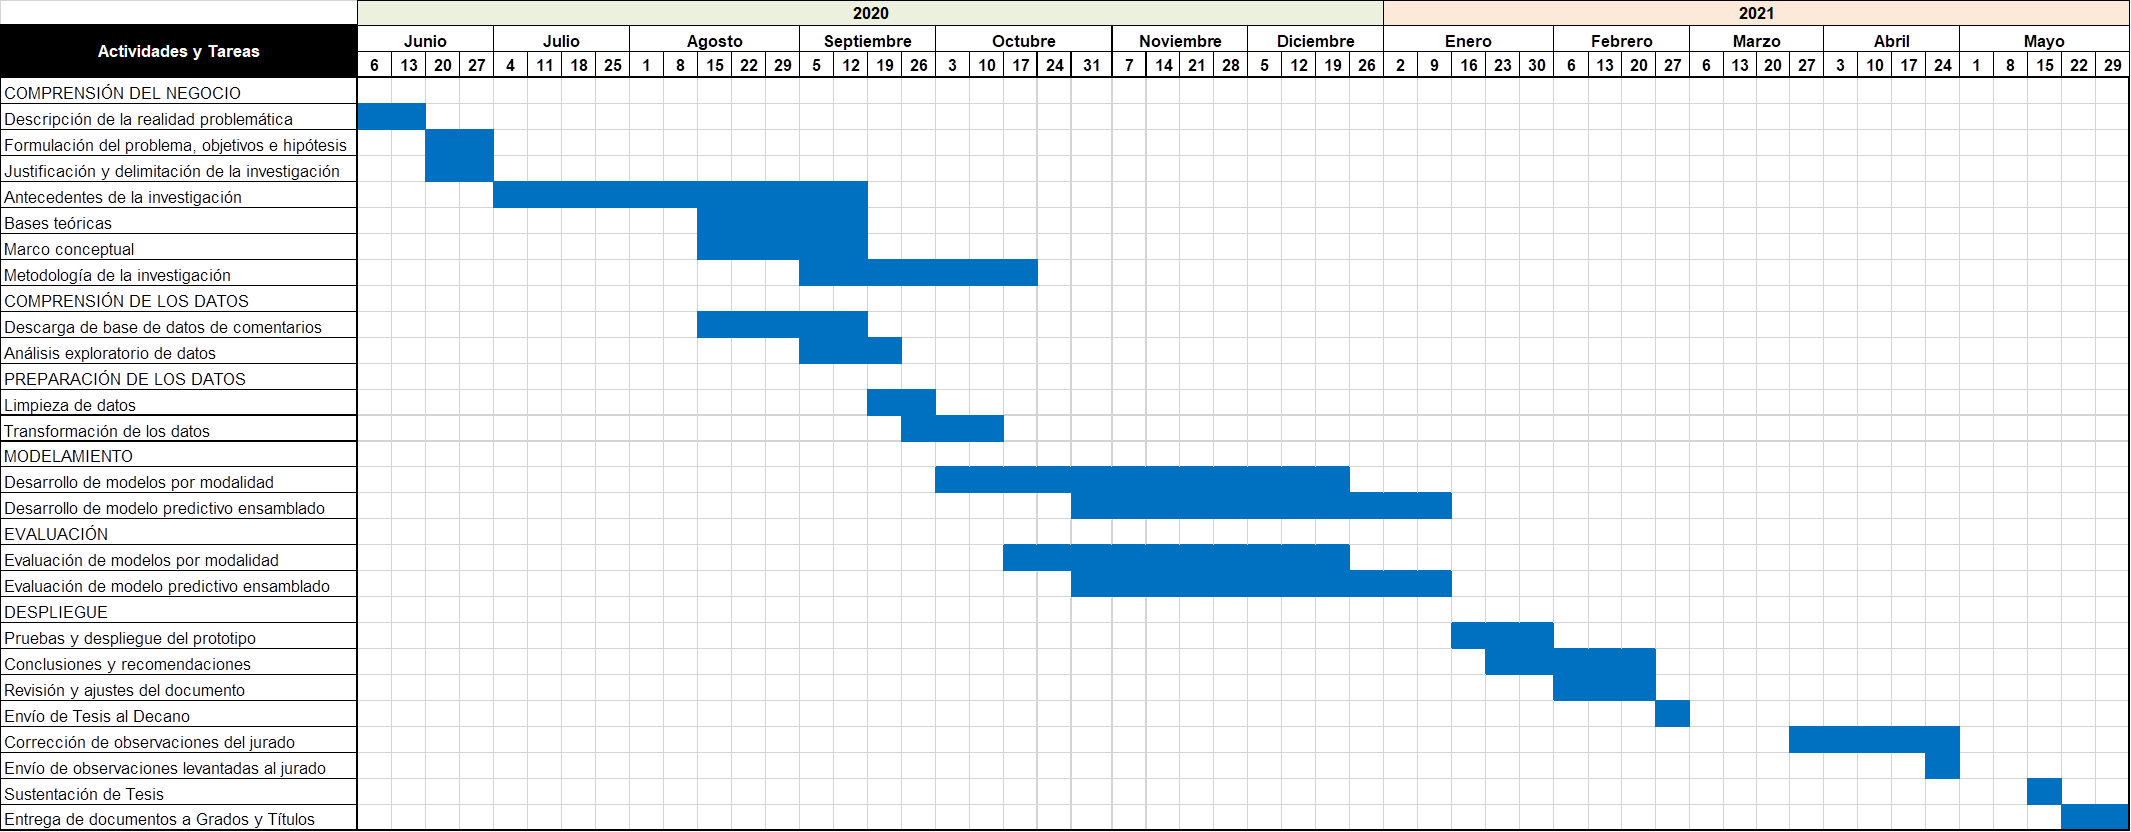
\includegraphics[width=1.1\textwidth]{3/figures/cronograma.png}
		\caption[Cronograma de actividades de la investigación]{Cronograma de actividades de la investigación.\\
		Fuente: Elaboración propia}
		\label{3:fig8}
	\end{center}
\end{figure}

La partida presupuestal de todo el proyecto se divide en dos partes: los costos personales del autor y los costos de las herramientas para la operación del proyecto.

Los costos personales del autor del trabajo de tesis se muestran en la Tabla \ref{3:table9}. Estos incluyen las herramientas adquiridas antes del inicio de la investigación como la laptop, así como los pagos de servicios generales y del trámite de elaboración y sustentación pública de Tesis. Se menciona la cantidad de horas utilizadas por el autor para el desarrollo del trabajo; sin embargo no se considera un valor monetario por cada unidad al ser un valor incalculable.

\begin{table}[h!]
	\caption[Presupuesto de los costos personales del autor]{Presupuesto de los costos personales del autor.}
	\label{3:table9}
	\centering
	\small
	\begin{tabular}{lcrr}
		\rowcolor[HTML]{010066} 
		\multicolumn{1}{c}{\cellcolor[HTML]{010066}{\color[HTML]{FFFFFF} \textbf{Item}}} & \multicolumn{1}{c}{\cellcolor[HTML]{010066}{\color[HTML]{FFFFFF} \textbf{Tiempo usado (horas)}}} & \multicolumn{1}{c}{\cellcolor[HTML]{010066}{\color[HTML]{FFFFFF} \textbf{Costo (soles)}}} & \multicolumn{1}{c}{\cellcolor[HTML]{010066}{\color[HTML]{FFFFFF} \textbf{Subtotal}}}     \\
		\rowcolor[HTML]{DAE8FC} 
		\multicolumn{4}{l}{\cellcolor[HTML]{DAE8FC}\textbf{Recursos materiales}}                                                  \\
		Laptop Lenovo ideapad 330 Core i7 8va Gen  &  & S/.4,500.00 & S/.4,500.00 \\
		\rowcolor[HTML]{DAE8FC} 
		\multicolumn{4}{l}{\cellcolor[HTML]{DAE8FC}\textbf{Pagos del trámite de elaboración y sustentación pública de Tesis}}                                                                                                                                                                                                                                                \\
		Derecho de inscripción de tema de investigación &  & S/.800.00 & S/.800.00 \\
		Reserva del tema de tesis  &  & S/.2,700.00 & S/.2,700.00 \\
		Derecho de sustentación                                                          & & S/.1,500.00                                                                               & S/.1,500.00                                                                              \\
		\rowcolor[HTML]{DAE8FC} 
		\multicolumn{4}{l}{\cellcolor[HTML]{DAE8FC}\textbf{Recursos humanos}} \\
		Avance de tesis                                                                  & \multicolumn{1}{r}{900}                                                                    & Incalculable                                                                              & -                                                                                        \\
		\rowcolor[HTML]{DAE8FC} 
		\multicolumn{4}{l}{\cellcolor[HTML]{DAE8FC}\textbf{Servicios generales}}                                                   \\
		Internet + luz (7 meses)                                                         & \multicolumn{1}{r}{110}                                                                    & S/.80.00                                                                                  & S/.560.00                                                                              \\
		\rowcolor[HTML]{303498} 
		{\color[HTML]{FFFFFF} \textbf{Total}} & {\color[HTML]{FFFFFF} } & \multicolumn{1}{l}{\cellcolor[HTML]{303498}{\color[HTML]{FFFFFF} }} & \multicolumn{1}{l}{\cellcolor[HTML]{303498}{\color[HTML]{FFFFFF} \textbf{S/.10,060.00}}}
	\end{tabular}
	\par	%%Salto de linea
	\bigskip
	\begin{flushleft}	%%Alinear a la izquierda sin justificar
		\small Fuente: Elaboración propia.
	\end{flushleft}
\end{table}

Asimismo, también se contemplan los costos por uso de servicios en la nube como parte de la extracción de comentarios desde servidores en Google Cloud Platform (GCP) y desarrollo de modelos en Google Colab Pro en la Tabla \ref{3:table10}.

\begin{table}[h!]
	\caption[Presupuesto de los costos de las herramientas para el proyecto]{Presupuesto de los costos de las herramientas para el proyecto.}
	\label{3:table10}
	\centering
	\small
	\begin{tabular}{lcrcr}
		\rowcolor[HTML]{010066} 
		\multicolumn{1}{c}{\cellcolor[HTML]{010066}{\color[HTML]{FFFFFF} \textbf{Item}}} & \multicolumn{1}{c}{\cellcolor[HTML]{010066}{\color[HTML]{FFFFFF} \textbf{Unidades}}} & \multicolumn{1}{c}{\cellcolor[HTML]{010066}{\color[HTML]{FFFFFF} \textbf{Costo (dólares)}}} & \multicolumn{1}{l}{\cellcolor[HTML]{010066}{\color[HTML]{FFFFFF} \textbf{Horas}}} & \multicolumn{1}{c}{\cellcolor[HTML]{010066}{\color[HTML]{FFFFFF} \textbf{Subtotal}}} \\
		\rowcolor[HTML]{DAE8FC} 
		\multicolumn{4}{l}{\cellcolor[HTML]{DAE8FC}\textbf{Google Cloud Platform}}                                                                                                                                                                                                                                                                                & \textbf{-\$98.56}                                                                    \\
		Instancia VM Ubuntu (g1-small, 12GB RAM) & 1 & \$0.021 & 310 & \$6.51 \\
		Imagen de instancia Ubuntu & 8 & \$0.02 & 306 & \$48.96                                                                              \\
		Instancia VM de Windows Server 2019 (4GB RAM) & 1 & \$0.086 & 300 & \$25.80                                                                              \\
		Costo por instancias encendidas & 10 & & & \$3.41                                                                               \\
		Uso de instancias posteriormente eliminadas & & & & \$95.88                                                                              \\
		Pago mensual (luego de aceptar mejora de plan) & 4 & \$5.22 & & \$20.88                                                                              \\
		Crédito de \$300.00 por 12 meses & 1 & -\$300.00 & & -\$300.00                                                                            \\
		\rowcolor[HTML]{DAE8FC} 
		\multicolumn{4}{l}{\cellcolor[HTML]{DAE8FC}\textbf{Google Colab Pro}}                                                                                                                                                                                                                                                                                     & \textbf{\$49.95}                                                                     \\
		Pago mensual (luego de aceptar mejora de plan) & 5 & \$9.99 & \multicolumn{1}{l}{} & \$49.95                                                                              \\
		\rowcolor[HTML]{303498} 
		{\color[HTML]{FFFFFF} \textbf{Total a pagar}} & {\color[HTML]{FFFFFF}} & \multicolumn{1}{l}{\cellcolor[HTML]{303498}{\color[HTML]{FFFFFF} }} & \multicolumn{1}{l}{\cellcolor[HTML]{303498}} & {\color[HTML]{FFFFFF} \textbf{\$49.95}}                                             
	\end{tabular}
	\par	%%Salto de linea
	\bigskip
	\begin{flushleft}	%%Alinear a la izquierda sin justificar
		\small Fuente: Elaboración propia.
	\end{flushleft}
\end{table}

Los montos totales por el uso de instancias creadas en GCP son descontados de los \$300.00 en crédito gratuito válidos por 12 meses (a la fecha en que se desarrolló la investigación) \parencite{ot_googlecloud_freetrial}, recibidos inicialmente desde el 12 de agosto del 2020 (fecha de inscripción) para poder ser usados como versión de prueba. A partir del siguiente mes, se mejoró el plan para habilitar más servicios (por ejemplo, máquina virtual en Windows) y comenzó a facturarse \$5.22 mensualmente.